\documentclass[journal]{IEEEtran}
\usepackage{fancyhdr}
\usepackage{graphicx}
\usepackage[spanish]{babel}
\usepackage[utf8]{inputenc}
\usepackage{color}
\usepackage{hyperref}
\usepackage{lipsum}
\usepackage{tikz,amsmath,amssymb,amsthm,lipsum}
\usetikzlibrary{matrix}




\newcommand{\MYhead}{\smash{\scriptsize
\hfil\parbox[t][\height][t]{\textwidth}{\centering\begin{picture}(0,0) \put(-30,-13){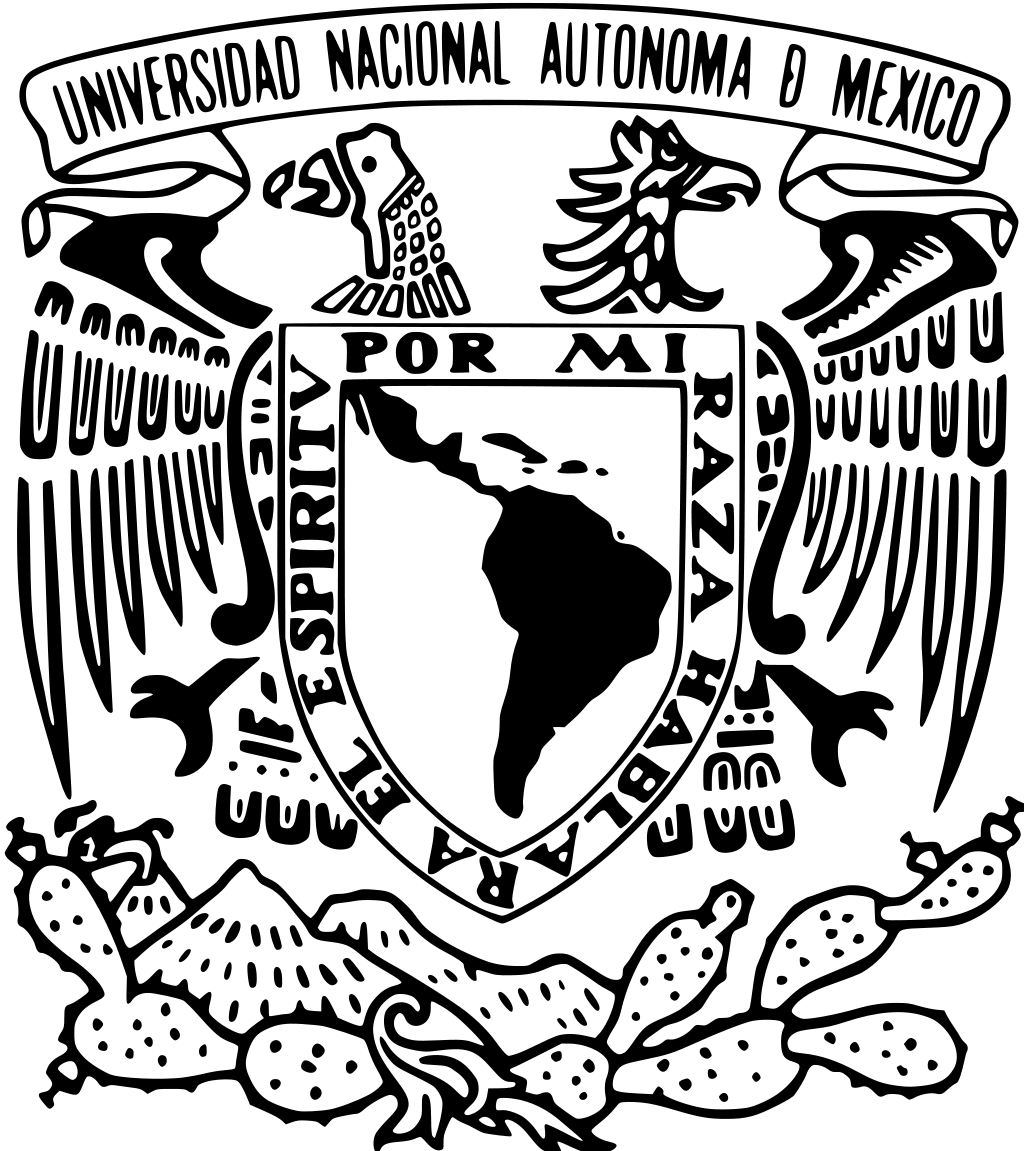
\includegraphics[width=12mm]{Imágenes/uman.png}} \end{picture}
\hspace{7.9cm} Pong en Python\\ \hspace{2cm}
\hspace{6.2cm} UNIVERSIDAD NACIONAL AUTÓNOMA DE MÉXICO \\
\underline{\hspace{ \textwidth}}}\hfil\hbox{}}}
\makeatletter


\def\ps@IEEEtitlepagestyle{%
\def\@oddhead{\MYhead}%
\def\@evenhead{\MYhead}}%
\makeatother



%______________________________________INICIO DEL DOCUMENTO________________________________%
\begin{document}

\title{\large{\textbf{Programando el videojuego "Pong" en Python usando la libreria «turtle»}}}
\author{Perez Erick,~
        Cruz Flores Angel Daniel,~
        Nava Villavicencio Abraham,~
        y López Bello Rebeca\\
				Profesor: Pedro Arturo Flores Silva \\\vspace{0.5cm}
\small{04 de diciembre de 2022}
\thanks{El presente documento corresponde a la práctica de [] presentado en la UNAM durante el periodo 2022-2}}



\maketitle

\begin{abstract}
Python es un lenguaje de alto nivel de programación interpretado cuya filosofía hace hincapié en la legibilidad de su código, se utiliza para desarrollar aplicaciones de todo tipo como Instagram, Netflix, Spotify, Panda3D, entre otros.\\
La finalidad de este proyecto es evaluar la cantidad de conociciento adquirido durante el ciclo escolar universitario de los estudiantes de computación mediante la creación del juego "Pong" en python, en el cual se vio el funcionamiento básico de python; la sintaxis que usa, algunos de los problemas que se pueden resolver usando la programación y otras caracteristicasutiles del mismo.
\end{abstract}

%%%%%%%%%%%%%%%%%%%%%%%%%%%%%%%%%%%%%%%%% INTRODUCCIÓN %%%%%%%%%%%%%%%%%%%%%%%%%%%%%%%%%%%%%%%%%%%%%

\section{Introducción}
Lanzado en 1972 por la compañía «Atari«, el «Pong» está considerado por muchos como el principal iniciador de la industria del videojuego. Su dinámica era bien sencilla: El jugador controlaba en el juego una paleta moviéndola verticalmente en la parte izquierda de la pantalla pudiendo competir tanto contra un oponente controlado por computadora, como contra jugador humano que controlaba una segunda paleta en la parte opuesta. Dichos jugadores podían usar las paletas para pegarle a la pelota hacia un lado u otro. El objetivo consistía en que uno de los jugadores obtuviera más puntos que el oponente al finalizar el juego. Puntos que se obtenían cuando el jugador adversario fallaba al devolver la pelota. Pues bien, en el artículo de hoy nos proponemos a programar nuestra propia versión de aquel juego, en Python, valiéndonos dela librería «turtle«.

%%%%%%%%%%%%%%%%%%%%%%%%%%%%%%%%%%%%%%%%%% DESARROLLO %%%%%%%%%%%%%%%%%%%%%%%%%%%%%%%%%%%%%%%%%%%%%%

\section{Desarrollo experimental}	
Como es habitual, iniciaremos la elaboración de nuestro código realizandolas importaciones pertinentes, es decir, la librería «turtle» para los gráficos.

\begin{figure}[ht]
    \centering
    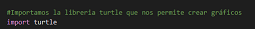
\includegraphics{Imágenes/1.png}
    \caption{Importamos la libreria}
    \label{fig:my_label}
\end{figure}

Realizada las importaciones de los recursos a emplear, empezaremos creando y configurando a nuestro gusto una ventana nueva que se iniciará cada vez que se ejecute el código.

\begin{figure}[ht]
    \centering
    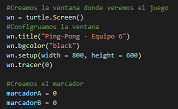
\includegraphics{Imágenes/2.png}
    \caption{Creación y configuración de la ventana y las variables marcadorA y marcadorB. }
    \label{fig:my_label}
\end{figure}

Como se ve, empezamos creando el área en el que se desarrollará el juego, usando el método «turtle.Screen()» cuyo título, color de fondo y dimensiones, estableceremos mediante los métodos «.title()«, «bgcolor()» y «setup()» respectivamente. Trasello, crearemos lasvariables «marcadorA» y «marcadorB» que con valor inicial 0, llevarán la cuenta de los puntos obtenidos por jugadores, (los cuales serán controladas mediante el teclado) que pasaremos a crear a continuación con el método «turtle.Turtle()«:

\begin{figure}[ht]
    \centering
    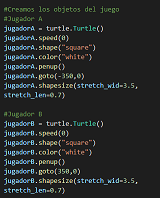
\includegraphics{Imágenes/3.png}
    \caption{Creación de los jugadores A y B}
    \label{fig:my_label}
\end{figure}

Nuestros jugadores, van a consistir en dos barras rectangulares colocadas a ambos extremos del área de juego. Por ello para su forma usaremos como base la figura del cuadrado (con «shape(«square»)«) cuyas dimensiones definiremos con el método«shapesize()«, su color con el método «color()» y su posición inicial, con «goto()«.\\

\begin{figure}[ht]
    \centering
    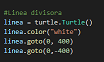
\includegraphics{Imágenes/4.png}
    \caption{Creación de la Linea divisora}
    \label{fig:my_label}
\end{figure}

Como observamos en la figura 4, el siguiente elemento gráfico que introduciremos es la línea divisoria del área de juego. Para ello usaremos los mismos métodos que empleamos para los jugadores, solo que aquí usaremos un color distinto, la posición base de las misma será el centro del área de juego («goto(0,0)«) y su alto y ancho será bastante mayor y menor respectivamente.\\



El siguiente elemento gráfico que vamos a incluir es la pelota. La cual va a consistir en un círculo posicionado inicialmente en el centro del área de juego:

\begin{figure}[ht]
    \centering
    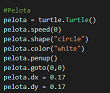
\includegraphics{Imágenes/5.png}
    \caption{Creación de la pelota}
    \label{fig:my_label}
\end{figure}

Como se ve, volvemos a usar los métodos que utilizamos para los elementos anteriores, solo que en este caso añadimos tres variables. Por una parte, las variables «pelota.dx» y «pelota.dy» con las que definiremos el espacio en pixeles que tanto en el eje «x» como en el eje «y«, va a avanzar nuestra pelota en su movimiento (determinando la fluidez del mismo), en estecaso fue de 0.17.\\


Finalmente, el último elemento gráfico es el contador de puntos. Introduciremos dicho texto mediante el método «.write()» al que pasaremos el texto en cuestión, la alineación y la fuente tipográfica:

\begin{figure}[ht]
    \centering
    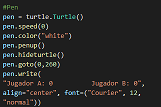
\includegraphics{Imágenes/6.png}
    \caption{Creación del marcador}
    \label{fig:my_label}
\end{figure}

Con esto ya tendríamos creados, con su configuración inicial, los elementos gráficos de nuestro juego. Los cuales, en pantalla se verán así al iniciarel programa:

\begin{figure}[ht]
    \centering
    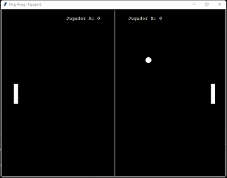
\includegraphics{Imágenes/7.png}
    \caption{Caption}
    \label{fig:my_label}
\end{figure}

Lo que toca ahora es definir las distintas funciones que gobernarán el comportamiento de los distintos elementos creados (Jugadores, pelota y el marcador) en función de los eventos que introduzcamos a través del teclado. Empezaremos esta explicación por el control de los jugadores:

\begin{figure}[ht]
    \centering
    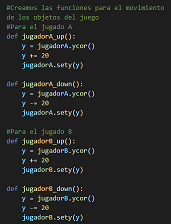
\includegraphics{Imágenes/8.png}
    \caption{Control de los jugadores}
    \label{fig:my_label}
\end{figure}

Tenemos aquí cuatro funciones con las que controlaremos el movimiento hacia arriba y hacia abajo de cada una de las palas. Puesto que el movimiento de las mismas es exclusivamente vertical, vamos a usar la variable «y» que será igual a coordenada «y» en la que, en cada momento, se encuentre nuestra pala (dicho punto se obtendrá con «jugadorB.ycor()«). De modo que cada vez que se ejecute alguna de estas funciones el valor de «y» se modificará en 20 unidades más («y += 20«) cuandola función sea para mover la pala hacia abajo (funciones «jugadorA\_down()» y «jugadorB\_down()«), y en 20 unidades menos («y -= 20«) cuando el movimiento sea hacia arriba («jugadorA\_up()» y «jugadorB\_up()«). Después de variar el valor de «y» se actualizará la posición del jugador con el método «sety()«.\\

Como ya hemos dicho, estas son las funciones que gobernarán el comportamiento de los elementos gráficos de nuestra área de juego. No obstante hay que recordar que la ejecución de algunas de ellas (concretamente lascuatro que mueven los jugadores hacia arriba y haciaabajo responde a determinados eventos introducidos mediante el teclado. Por ello usaremos un método («.listen()«) que pondrá al programa en «escucha» de las teclas que pulsemos del teclado:

\begin{figure}[ht]
    \centering
    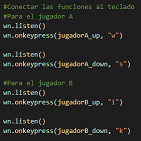
\includegraphics{Imágenes/9.png}
    \caption{Registrar eventos del teclado}
    \label{fig:my_label}
\end{figure}

Una vez iniciada la escucha el teclado, usaremos el método «onkeypress()» pasándole el nombre de la función que se ha de ejecutar y la tecla o evento que la ejecutará. De modo que tal y como lo hemos configurado, las teclas «w» y «s» moverán al jugador A (la de la izquierda) hacia arriba y abajo respectivamente. Por otra parte las teclas «i» y «k» lo mismo respecto al jugador B (la de la derecha).\\

Y finalmente, ejecutaremos un «while» que contendrá el desarrollo mismo del juego en el que definiremos el comportamiento y movimiento de la pelota en función de su posición respecto a los jugadores (de modo que por ejemplo, si entra en contacto con los jugadores, inicie un movimiento de retroceso):

\begin{figure}[ht]
    \centering
    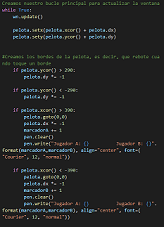
\includegraphics{Imágenes/10.png}
    \caption{Función while con el desarrollo del mismo juego}
    \label{fig:my_label}
\end{figure}

Como se ve en la imagen, durante el desarrollo de la partida, la pelota se moverá por el área de juego mediante la función «setx()» (para el eje horizontal) y «sety()» que tendrán como argumento el resultado de sumar al valor actual de posición el valor de «pelota.dx» y «pelota.dy» (que recordaremos que era de 0.17). En el transcurso de dicho desplazamiento por pantalla pueden darse dos circunstancias distintas: Que la pelota entre en contacto con alguna de los jugadores (en cuyocaso simularemos el retroceso de la misma tanto en su dirección como en su sentido. Algo parecido sucederá si la pelota entra en contacto con alguno de los bordes superior e inferior del área de juego. La otra eventualidad es que la pelota rebase a alguna de los jugadpres (lo que supone un punto más para el contrario). En ese caso se incrementará e 1, el valor de la variable «marcadorA» o «marcadorB» y se actualizará el texto que muestra en pantalla dicho resultado.\\

Esro se hace gracias al comadno pen.write, en la cual definimos un texto en el cual incluimos la variable masrcadorA y marcadorB, la cual indicamos al principio su valor es igual a cero, sin embargo, también definimos que, cada vez que la pelota toca, ya sea el borde izquierdo o derecho, el contador aumente uno, respectivamente, dependiento del borde que ha tocado.\\

La figura 11 indica quem cuadno la pelota toca a cualquier jugaro, entonces vaya al lado contrario.\\

\begin{figure}[ht]
    \centering
    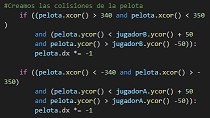
\includegraphics{Imágenes/11.png}
    \caption{Condicional if que indica a la pelota como moverse cuando colisiona con los jugadores}
    \label{fig:my_label}
\end{figure}

Finalmente, el juego se ve así:

\begin{figure}[ht]
    \centering
    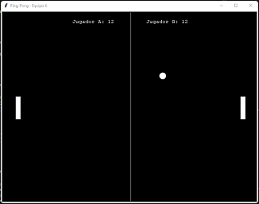
\includegraphics{Imágenes/12.png}
    \caption{Juego Final}
    \label{fig:my_label}
\end{figure}


\section{Resultados y análisis de resultados}
El resultado fue el esperado, fuimos capaces de replicar el juego Pong con gran exactitud, a excepción del sonido que no pudimos adquirirlo (o por lo menos de forma legal); sin embargo el juego fuera de ese detalle o de jugar contra la maquina que tiene diferentes dificultades (que por cirto no estaba dentro de los objetivos ya que una de las finalidades era el poder divertirse y pasar el rato jugando ya sea solo o con amigos) es una replcia de muy buena calidad, cuenta con un marcador que mantiene el puntaje de cada jugadorademas de que se actualiza cada vez que se anota un nuevo punto que sucede cuando la pelota alcanza o supera el limite determinado de pixeles y la secuencia se reinicia mandando a la pelota de vuelta al centro para la siguiente ronda, las paletas tambien están condicionadas a un area predeterminada para evitar accidentes que puedan suceder y afectar la jugabilidad, de la misma manera es sencillo reprogramarlo para añadir dificultad o restarsela, ya sea reduciendo o aumentando el tamaño de las paletas, o cambiando la velocidad de la pelota, o incluso reduciendo las dimensiones del cuadro donde se desarrolla el juego lo cual está indicado en el mismo programa y basta con cambiar unos cuantos valores para poder personalizar lo más posible el juego a las preferencias del usuario, siendo el programa una gran alternativa cuando no te puedes conectar a la red o simplemente no quieres instalar un juego o emulador que abarquen mucho espacio en la memoria de tu ordenador. 

\section{Conclusiones}
A lo largo de este proyecto pudimos observar que aunque la sintaxis del programa es sencilla, hay muchisimas cosas que aprender para poder llegar a ser un buen programador de python.
A pesar de que tuvimos algunos tropiezos al desarrollar este proyecto pudimos  solucionarlos y aprender de ellos trabajando en equipo, logrando concliur satisfactoriamente este tranajo, de el proceso nos llevamos más conocimiento a cerca de las bibliotecas que se pueden usar, el como funcionan y para que sirven, aunque reiteramos falta mucho por aprender de este lenguaje, pero ya estamos mas cerca que cuando empezamos.


\begin{thebibliography}{1}

\bibitem{Fuente 1}
Mundo Python.(2019). \emph{Como programar pong en python para principianetes(y en 120 lineas de código)}. recuperado el 4 de diciembre de 2022 de: https://www.youtube.com/watch?v=o9ddr3J7FY8

\bibitem{Fuente 2}
Sintes,M.(s/f). \emph{Gráficos: el módulo turtle (1)}. Recuperado el 4 de diciembre de 2022 de https://www.mclibre.org/consultar/python/lecciones/python-turtle-1.html
  \end{thebibliography}

\end{document}